\documentclass[../DoAn.tex]{subfiles}
\begin{document}

Chương này trình bày thiết kế của hệ thống, bắt đầu từ phân tích yêu
cầu và kiến trúc tổng thể hai giai đoạn, rồi đi vào thiết kế giai đoạn
phân tích tĩnh, giai đoạn phân tích động và pipeline tích hợp.

\section{Phân tích yêu cầu}
\label{section:3.1}

Trước khi đi vào thiết kế chi tiết, cần xác định rõ các yêu cầu mà hệ
thống phải đáp ứng, vì đây vừa là định hướng cho các quyết định thiết
kế, vừa là tiêu chí để đánh giá hệ thống về sau. Các yêu cầu được phân
thành hai nhóm. Yêu cầu chức năng mô tả những chức năng mà hệ thống
cung cấp. Yêu cầu phi chức năng quy định các ràng buộc về chất lượng
vận hành --- như tính cô lập của môi trường thực thi, mức độ tự động
hóa và khả năng chịu lỗi khi một giai đoạn gặp sự cố.

\subsection{Yêu cầu chức năng}
\label{section:3.1.1}
Bảng~\ref{tab:functional_req} liệt kê các yêu cầu chức năng của hệ thống.
\begin{table}[H]
\centering
\caption{Yêu cầu chức năng của hệ thống.}
\label{tab:functional_req}
\begin{tabular}{|c|p{12cm}|}
\hline
\multicolumn{1}{|c|}{\textbf{Mã}} & \multicolumn{1}{c|}{\textbf{Yêu cầu}} \\
\hline
F1 & Nhận tệp PE 32/64-bit (\texttt{.exe}, \texttt{.dll}) làm đầu vào \\
\hline
F2 & Trích xuất vector đặc trưng 2.381 chiều từ cấu trúc tệp PE mà không thực thi tệp \\
\hline
F3 & Phân loại tệp là malware hoặc benign, kèm xác suất dự đoán từ mô hình học máy đã huấn luyện \\
\hline
F4 & Thực thi mẫu trong môi trường sandbox Windows VM cô lập với mạng giả lập \\
\hline
F5 & Thu thập sự kiện hệ thống từ Sysmon và SilkETW trong suốt quá trình thực thi \\
\hline
F6 & Trích xuất IOC gồm địa chỉ IP, tên miền, URL, tệp được tạo và bị xóa,
     khóa registry, câu lệnh, named pipe, PID tiến trình bị tiêm mã và giá trị băm SHA-256 \\
\hline
F7 & Xây dựng cây tiến trình và chuỗi hành vi theo thứ tự thời gian \\
\hline
F8 & Ánh xạ hành vi quan sát được sang các kỹ thuật MITRE ATT\&CK tương ứng \\
\hline
F9 & Xuất báo cáo phân tích dạng JSON \\
\hline
\end{tabular}
\end{table}
\subsection{Yêu cầu phi chức năng}
\label{section:3.1.2}
Bảng~\ref{tab:nonfunctional_req} liệt kê các yêu cầu phi chức năng của hệ thống.
\begin{table}[H]
\centering
\caption{Yêu cầu phi chức năng của hệ thống.}
\label{tab:nonfunctional_req}
\begin{tabular}{|c|p{12cm}|}
\hline
\multicolumn{1}{|c|}{\textbf{Mã}} & \multicolumn{1}{c|}{\textbf{Yêu cầu}} \\
\hline
NF1 & Mẫu độc hại chỉ được thực thi bên trong máy ảo, không bao giờ chạy trực 
      tiếp trên máy chủ phân tích \\
\hline
NF2 & VM được khôi phục về snapshot sạch \texttt{Clean\_Base} trước mỗi lần
      phân tích, đảm bảo tính độc lập giữa các lần chạy \\
\hline
NF3 & Pipeline vận hành hoàn toàn tự động từ khâu nhận tệp đến khâu xuất
      báo cáo, không yêu cầu can thiệp thủ công \\
\hline
NF4 & Nếu giai đoạn phân tích động thất bại, hệ thống vẫn lưu kết quả phân 
      tích tĩnh và xuất báo cáo với thông tin hiện có \\
\hline
NF5 & Thời gian thu thập sự kiện trong giai đoạn động có thể cấu hình, mặc định là 120 giây \\
\hline
\end{tabular}
\end{table}
\section{Kiến trúc tổng thể}
\label{section:3.2}

Hình~\ref{fig:system_architecture} minh họa kiến trúc tổng thể của hệ
thống, gồm hai giai đoạn phân tích tĩnh và động.
\begin{figure}[H]
  \centering
  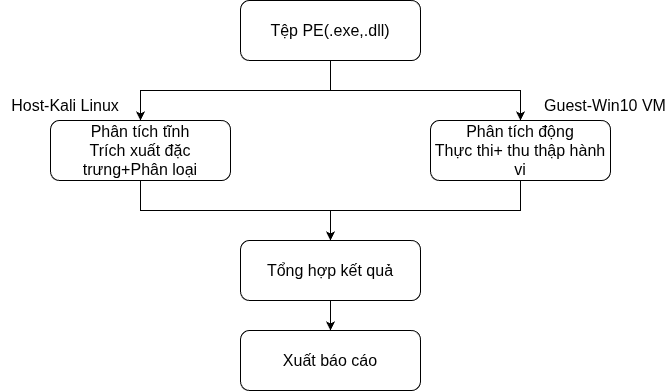
\includegraphics[width=0.9\linewidth]{Hinhve/Pic6Tongquan.png}
  \caption{Kiến trúc tổng thể của hệ thống phân tích phần mềm độc hại.}
  \label{fig:system_architecture}
\end{figure}
Giai đoạn phân tích tĩnh chạy trên máy chủ Kali Linux: trích xuất
vector đặc trưng từ cấu trúc tệp PE, sau đó đưa qua mô hình phân 
loại để trả về nhãn cùng xác suất dự đoán. Thuật toán được sử dụng 
là LightGBM, được lựa chọn dựa trên kết quả so sánh thực nghiệm với 
Random Forest và XGBoost trên cùng bộ đặc trưng (trình bày tại 
Chương~\ref{chapter:Experiment}).
 
Giai đoạn phân tích động chạy trong máy ảo Windows~10 trên VirtualBox:
khôi phục môi trường về trạng thái sạch, thực thi mẫu trong điều kiện
mạng giả lập, đồng thời thu thập sự kiện hệ thống qua Sysmon và
SilkETW. Sau khi thu thập xong, dữ liệu sự kiện được kéo về máy chủ
để xử lý thành chuỗi hành vi, IOC và ánh xạ MITRE ATT\&CK.

Khi cả hai giai đoạn hoàn tất, hệ thống tổng hợp kết quả và xuất
báo cáo JSON duy nhất chứa kết luận, bằng chứng hành vi, cây tiến trình và
các chỉ số xâm phạm.
\section{Thiết kế giai đoạn phân tích tĩnh}
\label{section:3.3}
Giai đoạn phân tích tĩnh phân loại tệp PE dựa hoàn toàn vào đặc trưng
cấu trúc mà không thực thi tệp. Hình~\ref{fig:static-inference} mô tả
luồng xử lý: tệp PE qua bộ trích xuất đặc trưng để tạo vector, sau đó
mô hình phân loại trả về nhãn dự đoán cùng xác suất tương ứng.
\begin{figure}[H]
    \centering
    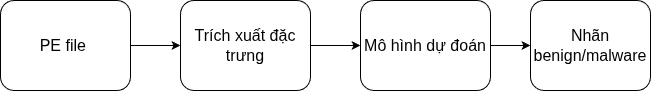
\includegraphics[width=\linewidth]{Hinhve/Pic7Static.png}
    \caption{Luồng phân tích tĩnh khi tiếp nhận tệp đầu vào}
    \label{fig:static-inference}
\end{figure}
Để xây dựng mô hình phân loại trên, hệ thống trải qua quy trình huấn luyện 
gồm năm bước như thể hiện trong Hình~\ref{fig:static-training}: thu thập và 
xây dựng tập dữ liệu, trích xuất đặc trưng, huấn luyện sơ bộ để tính độ quan 
trọng đặc trưng, lựa chọn tập con đặc trưng tối ưu, và huấn luyện lại mô hình 
cuối dựa trên tập đặc trưng đã chọn.
\begin{figure}[H]
    \centering
    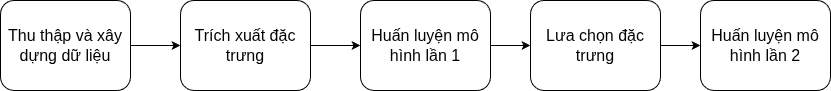
\includegraphics[width=\linewidth]{Hinhve/Pic8Model.png}
    \caption{Quy trình xây dựng mô hình phân loại tĩnh}
    \label{fig:static-training}
\end{figure}
\subsection{Thu thập và xây dựng tập dữ liệu}
\label{section:3.3.1}

Tập dữ liệu gồm hai lớp: khoảng 132.000 tệp mã độc thu thập từ
các kho lưu trữ công khai và khoảng 110.000 tệp lành tính từ phần
mềm hợp pháp và thành phần hệ điều hành Windows. Sau khi kiểm tra
hợp lệ PE, loại trùng lặp theo giá trị băm và tiền xử lý, tập dữ
liệu có hơn 201.000 mẫu phân bố gần cân bằng giữa hai lớp. Thống
kê chi tiết theo nguồn và bước tiền xử lý được trình bày tại
Chương~\ref{chapter:Implementation}.
\subsection{Trích xuất đặc trưng}
\label{section:3.3.2}

Mỗi tệp PE được chuyển đổi thành vector 2.381 chiều theo chín nhóm
đặc trưng EMBER (Bảng~\ref{tab:ember_features} trong Chương~\ref{chapter:Related_works}).
Các nhóm có kích thước cố định như entropy và header info được giữ
nguyên giá trị số. Các nhóm có độ dài thay đổi như danh sách hàm
import được chuẩn hóa về kích thước cố định qua kỹ thuật feature
hashing~\cite{weinberger2009}: mỗi tên hàm được băm thành một vị trí
trong mảng, nhờ đó mọi tệp PE đều tạo ra vector cùng kích thước.

\subsection{Huấn luyện mô hình}
\label{section:3.3.3}

Như minh họa trong Hình~\ref{fig:static-training}, quy trình huấn
luyện được thiết kế thành hai lần huấn luyện nối tiếp, với bước lựa
chọn đặc trưng đặt ở giữa: lần thứ nhất để chọn thuật toán phù hợp,
lần thứ hai để chọn tập đặc trưng tối ưu cho thuật toán đó. Việc tách
thành hai lần giúp mỗi quyết định được đưa ra độc lập và có cơ sở so
sánh rõ ràng.

Ở lần huấn luyện thứ nhất, ba thuật toán Random Forest, XGBoost và
LightGBM (Mục~\ref{section:2.3.2}) được huấn luyện trên cùng tập dữ
liệu và toàn bộ đặc trưng, trong cùng điều kiện. Nhờ giữ mọi yếu tố
giống nhau, khác biệt về kết quả chỉ phản ánh bản chất của từng thuật
toán, giúp việc lựa chọn được khách quan. Thuật toán cho hiệu năng tốt
nhất được giữ lại làm mô hình triển khai.

Ở lần huấn luyện thứ hai, số chiều đặc trưng được giảm bớt nhằm thu
được mô hình gọn và dễ diễn giải hơn mà vẫn duy trì hiệu năng. Các đặc
trưng được xếp hạng theo Importance Gain (Mục~\ref{section:2.3.3}) của
mô hình đã chọn, sau đó chỉ giữ lại nhóm đặc trưng quan trọng nhất để
huấn luyện lại. Thay vì ấn định trước một số chiều, hiệu năng được khảo
sát ở nhiều mức khác nhau nhằm tìm điểm bão hòa --- nơi việc thêm đặc
trưng gần như không còn cải thiện kết quả --- rồi chọn số chiều quanh
điểm đó.

Để kết quả đánh giá đáng tin cậy, mô hình không chỉ được kiểm tra trên
phần dữ liệu tách ra từ tập huấn luyện mà còn trên các tập dữ liệu độc
lập hoàn toàn, trong đó có một tập công khai thu thập từ nguồn khác.
Cách này cho phép đo khả năng tổng quát hóa của mô hình trên dữ liệu
ngoài phân phối huấn luyện, thay vì chỉ trên dữ liệu cùng nguồn. Mô
hình cuối còn được phân tích sâu hơn ở các khía cạnh như ngưỡng phân
loại, các trường hợp phân loại sai và mức đóng góp của từng nhóm đặc
trưng; toàn bộ kết quả được trình bày tại Chương~\ref{chapter:Experiment}.

\section{Thiết kế giai đoạn phân tích động}
\label{section:3.4}

Giai đoạn phân tích động thực thi mẫu nghi ngờ trong môi trường 
sandbox cô lập nhằm thu thập hành vi thực tế trong quá trình chạy, bổ 
sung cho kết quả phân loại tĩnh. Luồng xử lý gồm sáu bước như minh 
họa trong Hình~\ref{fig:dynamic_steps}: (1) thiết lập môi trường 
sandbox, (2) thực thi mẫu trong máy ảo, (3) thu thập sự kiện từ 
Sysmon và SilkETW, (4) chuẩn hóa và lọc nhiễu, (5) xây dựng cây tiến 
trình và chuỗi hành vi đồng thời trích xuất IOC, và (6) ánh xạ hành 
vi sang MITRE ATT\&CK. Tại mỗi bước, nếu xảy ra lỗi, hệ thống ghi
nhận và dừng giai đoạn động, kết quả phân tích tĩnh vẫn được giữ lại
(yêu cầu NF4).
\begin{figure}[H]
    \centering
    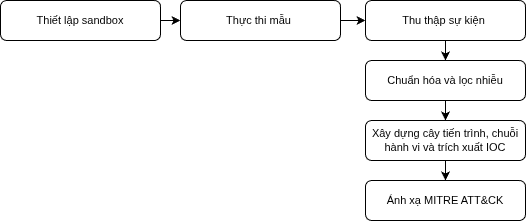
\includegraphics[width=\linewidth]{Hinhve/Pic10Dynamic.png}
    \caption{Luồng xử lý giai đoạn phân tích động.}
    \label{fig:dynamic_steps}
\end{figure}
\subsection{Thiết lập môi trường sandbox}
\label{section:3.4.1}

Môi trường phân tích động gồm hai thành phần: máy chủ phân tích 
(host) chạy Kali Linux và máy ảo (guest) chạy Windows~10 trên nền 
tảng VirtualBox, kết nối qua mạng host-only đảm bảo máy ảo chỉ giao 
tiếp được với host mà không truy cập trực tiếp ra Internet (yêu cầu 
NF1). Hình~\ref{fig:sandbox_arch} phác họa kiến trúc môi trường 
sandbox.
\begin{figure}[H]
    \centering
    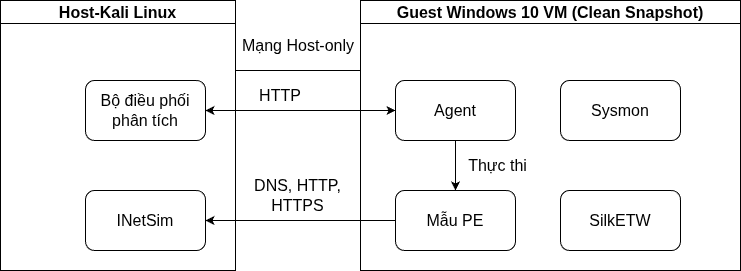
\includegraphics[width=\linewidth]{Hinhve/Pic11Sandbox.png}
    \caption{Kiến trúc môi trường sandbox.}
    \label{fig:sandbox_arch}
\end{figure}
Phía host triển khai INetSim — công cụ giả lập các dịch vụ mạng phổ 
biến như DNS, HTTP, HTTPS. Khi mã độc cố gắng kết nối ra ngoài, INetSim 
cung cấp phản hồi giả, nhờ đó hệ thống vừa quan sát được hành vi kết 
nối mạng của mẫu, vừa ngăn chặn rủi ro lây lan.

Phía guest được cài đặt sẵn ba thành phần: Sysmon giám sát sự kiện hệ
điều hành, SilkETW thu thập sự kiện từ .NET Runtime và một agent chạy
dưới dạng dịch vụ HTTP bên trong VM. Mẫu PE được tải lên VM thông qua
cơ chế Guest Additions của VirtualBox, cho phép truyền tệp trực tiếp
giữa host và guest. Agent đóng vai trò đầu mối điều khiển các tác vụ phân tích bên trong
VM, bao gồm thực thi mẫu, điều phối quá trình thu thập sự kiện và
chuyển kết quả về host. Toàn bộ quá trình phân tích động do đó được
điều khiển từ xa mà không cần tương tác trực tiếp với giao diện
Windows (yêu cầu NF3).

Trước mỗi lần phân tích, VM được khôi phục về snapshot sạch nhằm đảm
bảo mỗi mẫu được thực thi trong môi trường độc lập và không chịu ảnh
hưởng từ các lần chạy trước (yêu cầu NF2).

\subsection{Thực thi mẫu}
\label{section:3.4.2}

Sau khi môi trường sandbox được khởi tạo, mẫu PE được thực thi bên
trong máy ảo để tạo ra các hành vi có thể quan sát được. Quá trình
thực thi được điều phối hoàn toàn bởi Agent bên trong VM, không yêu
cầu tương tác thủ công với hệ điều hành (yêu cầu NF3).
Hình~\ref{fig:execution_flow} tóm tắt luồng xử lý của bước này.
\begin{figure}[H]
  \centering
  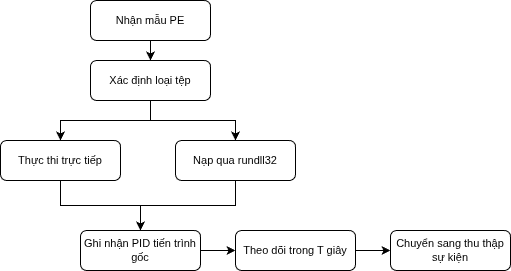
\includegraphics[width=\linewidth]{Hinhve/Pic12Execute.png}
  \caption{Luồng thực thi mẫu trong môi trường sandbox.}
  \label{fig:execution_flow}
\end{figure}
Agent thực thi mẫu theo cách phù hợp với định dạng: \texttt{.exe}
được khởi chạy trực tiếp; \texttt{.dll} nạp qua
\texttt{rundll32.exe}. Sau khi khởi chạy, Agent ghi nhận PID của
tiến trình gốc và chuyển cho bước thu thập sự kiện ở
Mục~\ref{section:3.4.3}.

Thời gian quan sát có thể cấu hình, mặc định 120 giây (yêu cầu
NF5). Khi hết thời gian hoặc gặp lỗi không thể phục hồi, hệ thống
kết thúc thực thi và giữ lại kết quả phân tích tĩnh theo yêu cầu
NF4.

\subsection{Thu thập sự kiện}
\label{section:3.4.3}

Trong suốt khoảng thời gian thực thi mẫu, hệ thống thu thập sự kiện
song song từ Sysmon và SilkETW như đã trình bày tại
Mục~\ref{section:2.4.2} và Mục~\ref{section:2.4.3}. Sysmon cung cấp
các sự kiện ở mức hệ điều hành như tạo tiến trình, thao tác tệp,
thay đổi registry và kết nối mạng; trong khi SilkETW ghi nhận các
sự kiện từ .NET Runtime nhằm quan sát các hoạt động thực thi bên
trong môi trường .NET.
\begin{figure}[H]
  \centering
  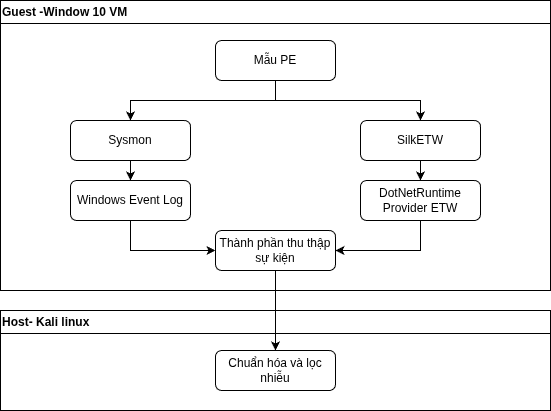
\includegraphics[width=0.8\linewidth]{Hinhve/Pic13Collection.png}
  \caption{Luồng thu thập sự kiện trong môi trường sandbox.}
  \label{fig:event_collection}
\end{figure}
Hình~\ref{fig:event_collection} mô tả kiến trúc thu thập sự kiện.
Trước khi mẫu được thực thi, bộ thu thập ghi nhận số thứ tự
(\texttt{RecordId}) mới nhất của kênh Sysmon làm mốc bắt đầu. Trong
quá trình thực thi, Sysmon được truy vấn định kỳ để lấy riêng các sự
kiện có \texttt{RecordId} lớn hơn mốc đó, không lẫn với lịch sử hệ
thống có trước phiên phân tích.

Sau khi Agent khởi chạy mẫu, PID của tiến trình gốc được chuyển cho
bộ thu thập; mỗi tiến trình con mới sinh ra tự động được thêm vào danh
sách theo dõi. Phạm vi giám sát do đó bao phủ toàn bộ cây tiến trình
của mẫu, loại bỏ các sự kiện từ tiến trình không liên quan.

Đối với SilkETW, quá trình ghi nhận sự kiện được khởi động đồng thời
với việc thực thi mẫu và kết thúc khi hết thời gian quan sát. SilkETW
lắng nghe provider \texttt{Microsoft-Windows-DotNETRuntime} và ghi các
sự kiện thu được ra tệp log.

Kết thúc giai đoạn thu thập, dữ liệu Sysmon được lưu dưới dạng
\texttt{sysmon\_\allowbreak events\allowbreak.jsonl}, còn dữ liệu ETW được lưu dưới dạng
\texttt{etw\_\allowbreak dotnet\allowbreak.json}. Hai tệp này được sử dụng làm đầu vào cho
bước chuẩn hóa và lọc nhiễu ở Mục~\ref{section:3.4.4}.

\subsection{Chuẩn hóa và lọc nhiễu}
\label{section:3.4.4}

Dữ liệu thu được từ Sysmon và SilkETW có định dạng và cấu trúc khác
nhau do được sinh ra từ hai cơ chế giám sát độc lập; trước khi phân
tích hành vi, hệ thống thực hiện bước chuẩn hóa nhằm chuyển toàn bộ
sự kiện về một mô hình dữ liệu thống nhất. Hình~\ref{fig:normalize}
minh họa luồng xử lý của bước này.
\begin{figure}[H]
  \centering
  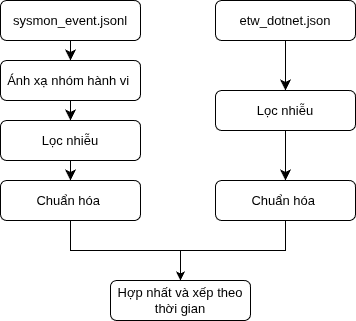
\includegraphics[width=0.65\linewidth]{Hinhve/Pic14Normalize.png}
  \caption{Luồng chuẩn hóa và lọc nhiễu dữ liệu.}
  \label{fig:normalize}
\end{figure}
Đối với Sysmon, mỗi sự kiện được ánh xạ từ Event ID sang nhóm hành vi
tương ứng như tạo tiến trình, thao tác tệp, thay đổi registry hoặc kết
nối mạng. Các trường dữ liệu quan trọng được trích xuất và chuẩn hóa
về cùng tên gọi. Đồng thời, hệ thống loại bỏ các sự kiện phát sinh từ
một số tiến trình hạ tầng đã biết của môi trường phân tích như Sysmon,
SilkETW, VirtualBox và các dịch vụ hệ thống không liên quan nhằm giảm
nhiễu trong dữ liệu đầu vào.

Đối với SilkETW, hệ thống chỉ giữ lại các sự kiện phản ánh hoạt động
nạp assembly (tải đơn vị mã .NET đã biên dịch vào bộ nhớ tại thời điểm
chạy) của .NET Runtime và loại bỏ các sự kiện phát sinh từ tiến trình
hạ tầng của môi trường phân tích. Các sự kiện còn lại được chuẩn hóa
về cùng mô hình dữ liệu thống nhất với Sysmon, đảm bảo hai nguồn có
thể được xử lý chung ở các bước sau.

Sau khi chuẩn hóa, mọi sự kiện đều được biểu diễn dưới dạng bản ghi
gồm thời gian xảy ra, nguồn sự kiện, loại hành vi, PID tiến trình và
dữ liệu chi tiết đi kèm. Toàn bộ sự kiện từ hai nguồn được hợp nhất,
sắp xếp theo thứ tự thời gian tăng dần và sử dụng làm đầu vào cho bước
xây dựng cây tiến trình, chuỗi hành vi và trích xuất IOC ở
Mục~\ref{section:3.4.5}.

\subsection{Xây dựng biểu diễn hành vi và ánh xạ MITRE ATT\&CK}
\label{section:3.4.5}

Tập sự kiện đã chuẩn hóa được tổ chức thành ba thành phần biểu diễn
hành vi: cây tiến trình, chuỗi hành vi và IOC.

Cây tiến trình được xây dựng từ quan hệ cha–con giữa các tiến trình,
lưu PID, đường dẫn thực thi, dòng lệnh và thời điểm khởi chạy. Chuỗi
hành vi gom các sự kiện thành mười một nhóm hành vi (tiến trình, tiêm
mã, nạp thư viện động, tệp, registry, mạng, DNS, named pipe, WMI,
.NET Runtime và nhóm khác) sắp xếp theo thứ tự thời gian. IOC được
trích xuất từ nội dung sự kiện, gồm mười danh mục: địa chỉ IP, tên
miền, URL, tệp được tạo, tệp bị xóa, khóa registry, câu lệnh, named
pipe, PID tiến trình bị tiêm mã và giá trị băm SHA-256.

Dựa trên ba thành phần trên, hệ thống áp dụng tập luật để ánh xạ
sang các kỹ thuật MITRE ATT\&CK. Mỗi luật kiểm tra điều kiện trên cây
tiến trình, chuỗi hành vi hoặc IOC; khi thỏa mãn, kỹ thuật ATT\&CK
tương ứng được ghi nhận. Các luật được tổ chức theo nhóm hành vi: thực
thi tiến trình, duy trì truy cập, tiêm mã, giao tiếp mạng và thực thi
.NET. Cách tiếp cận dựa trên luật cho phép bổ sung kỹ thuật mới hoặc
điều chỉnh tiêu chí nhận diện mà không cần huấn luyện lại mô hình.

\section{Thiết kế pipeline tích hợp}
\label{section:3.5}

Pipeline tích hợp phối hợp hai giai đoạn đã thiết kế tại
Mục~\ref{section:3.3} và Mục~\ref{section:3.4} để đưa ra kết quả phân
loại cuối cùng và xuất báo cáo; luồng xử lý tổng thể được minh họa
trong Hình~\ref{fig:pipeline_e2e}.
\begin{figure}[H]
  \centering
  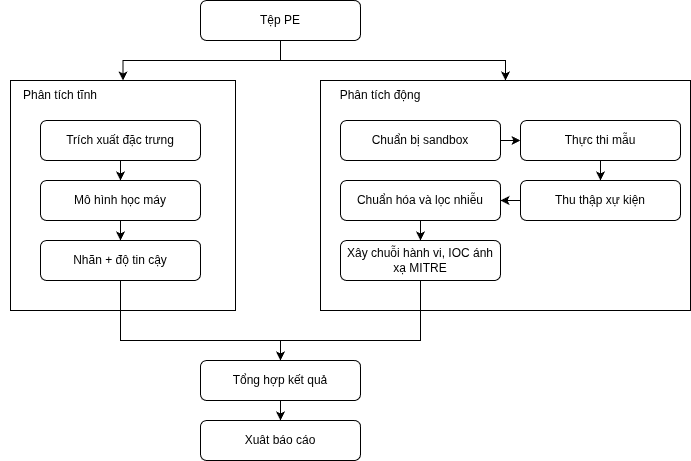
\includegraphics[width=1.0\linewidth]{Hinhve/Pic15Pipeline.png}
  \caption{Luồng xử lý end-to-end của pipeline tích hợp.}
  \label{fig:pipeline_e2e}
\end{figure}
Thiết kế hướng đến hai mục tiêu: rút ngắn thời gian tổng thể bằng cách
chạy song song hai giai đoạn, và đảm bảo kết quả luôn được xuất ra ngay
cả khi một giai đoạn gặp lỗi (yêu cầu NF4).
\subsection{Luồng xử lý end-to-end}
\label{section:3.5.1}
Ngay sau khi tiếp nhận tệp PE đầu vào, pipeline khởi động đồng
thời hai luồng độc lập. Luồng phân tích tĩnh trích xuất đặc trưng,
đưa qua mô hình học máy và trả về nhãn phân loại cùng xác suất
tương ứng. Luồng phân tích động lần lượt thực hiện các bước chuẩn
bị sandbox, thực thi mẫu, thu thập sự kiện, chuẩn hóa và lọc
nhiễu, sau đó xây dựng chuỗi hành vi, trích xuất IOC và ánh xạ
MITRE ATT\&CK. Hai luồng không phụ thuộc vào nhau; thời gian hoàn
thành của toàn pipeline xấp xỉ thời gian của luồng chậm hơn.

Sau khi cả hai luồng hoàn tất, hệ thống kết hợp kết quả ML và tín
hiệu phân tích động theo năm quy tắc để đưa ra kết luận cuối:
\texttt{malware}, \texttt{suspicious}, \texttt{benign} hoặc
\texttt{unknown}. Tín hiệu tiêm mã tiến trình được ưu tiên cao nhất
và có thể thay đổi kết luận của mô hình ML; nếu giai đoạn động không
thu được tín hiệu hành vi nào, hệ thống ghi cảnh báo nghi ngờ mẫu
dùng kỹ thuật lẩn tránh sandbox. Bảng quy tắc đầy đủ được trình bày
tại Chương~\ref{chapter:Implementation} (Bảng~\ref{tab:verdict-impl}).

\subsection{Cấu trúc báo cáo đầu ra}
\label{section:3.5.2}

Kết quả phân tích được tổng hợp thành một báo cáo JSON duy nhất gồm
năm nhóm. Ba nhóm đầu là kết quả chính: (1)~kết quả phân loại — nhãn
kết luận (\texttt{verdict}),
độ tin cậy tổng hợp (\texttt{confidence}), nhãn và xác suất thô của
mô hình ML; (2)~thông tin hành vi — chuỗi hành vi, cây tiến trình,
mô tả tóm tắt và danh sách kỹ thuật MITRE ATT\&CK; (3)~chỉ số xâm
phạm — địa chỉ IP, tên miền, URL, tệp được tạo, tệp bị xóa, khóa
registry, câu lệnh, named pipe, danh sách PID tiêm mã và giá trị băm
tệp liên quan. Hai nhóm còn lại phục vụ truy vết:
(4)~metadata phiên — SHA-256, kích thước mẫu, thời gian phân
tích và danh sách các giai đoạn đã hoàn thành; (5)~cảnh báo và lỗi
từ từng giai đoạn. Cấu trúc đầy đủ được trình bày tại
Chương~\ref{chapter:Implementation}.

Độ tin cậy tổng hợp khác với xác suất thô của mô hình ML: xác suất
thô phản ánh riêng kết quả giai đoạn tĩnh, còn độ tin cậy tổng hợp
có thể được điều chỉnh dựa trên kết quả phân tích động.

Điểm cốt lõi của thiết kế là kiến trúc hai giai đoạn chạy song song,
hợp nhất kết quả tĩnh và động theo một tập luật cố định, và luôn xuất
được báo cáo ngay cả khi một giai đoạn gặp lỗi. Cách hiện thực hóa
kiến trúc này được trình bày ở Chương~\ref{chapter:Implementation}.

\end{document}
